\documentclass[../main.tex]{subfiles}

\begin{document}

This chapter introduces previous work that has been undertaken on the subject of cookie notices and consequently, has influenced this project as well. Within the body of past work, 5 distinct subcategories have been identified and discussed further. These subcategories are summarised in the following list:

\begin{enumerate}
    \item Cookie banners and the privacy options that they offer to their visitors;
    \item Whether user location impacts cookie banners and privacy policies;
    \item The user interface (UI) of those cookie banners as well as dark patterns that websites employ to influence a user’s privacy choices;
    \item The effect that the GDPR had on cookie notices and how the privacy landscape changed;
    \item The prevalence of online tracking using cookies regardless of whether the user has agreed to be tracked or not. 
\end{enumerate}

\section{Cookie Notices \& Privacy Options}
Nowadays, cookie banners and privacy notices can be found in the vast majority of websites. Fundamentally, they are there to notify users that the website is using cookies, for advertising or other purposes, but also give users a means to manage their privacy settings or seek further information. 

However, not all websites provide their users with direct links to opt-out from tracking and instead are hiding those functions away from the cookie notices. This was researched by Habib et al. \cite{habib2019empirical} who conducted a 150-website analysis that aimed to determine the privacy mechanism and options available to users of those websites. Firstly, they wanted to know what are the options available to users in regards to email communication and targeted advertising. Secondly, they aimed to determine the ways that those websites present their privacy options to the users. Using the Alexa worldwide website rankings (\url{https://www.alexa.com/}), the authors used two thresholds for dividing and categorising those websites. Those were the top websites (ranks 1 - 200), middle websites (ranks 201 - 5,000) and finally bottom websites (ranks $>$ 5,000). Interestingly, the researchers found that privacy options are frequent within the surveyed websites. Specifically, they found that 89\% of websites offer email communication and targeted advertising opt-out options and 74\% of websites \say{had at least one data deletion mechanism}, which was higher than what other similar studies had found, as shown in Figure \ref{fig:habib_a}. Yet, direct opt-out links are found in only 27\% websites as depicted in Figure \ref{fig:habib_b} and therefore, multiple steps are needed for a user to be able to find a use that link. Moreover, they found that privacy policies contained missing, misleading and even unhelpful information. For instance, in 6 websites the text referred to opt-out but \say{that opt-out did not exist}. Moreover, the authors noted that in 15 websites, there were broken links or opt-out mechanisms and therefore, users could not opt-out even if they chose to.

\begin{figure}[ht]
    \centering
    \begin{subfigure}[b]{0.45\textwidth}
        \centering
        \begin{tikzpicture}
            \pie[radius=2,
                style=drop shadow,
                color={cyan, red}]{89/A, 11/B}
        \end{tikzpicture}
        \caption{The percentage of websites offering opt-out options (A) and the websites that do not offer one at all (B).}
        \label{fig:habib_a}
    \end{subfigure}
    \hfill
    \begin{subfigure}[b]{0.45\textwidth}
        \centering
        \begin{tikzpicture}
            \pie[radius=2,
                style=drop shadow,
                color={cyan, red}]{73/A, 27/B}
        \end{tikzpicture}
        \caption{The percentage of websites offering direct opt-out options (B) and the ones that require multiple steps (A).}
        \label{fig:habib_b}
    \end{subfigure}
    \caption{The opt-out options offered by the websites in Habib et al. sample.}
    \label{fig:habib}
\end{figure}

Regardless of whether websites offer cookie notices or not, websites in Europe have to ensure that their cookie notices follow the rules set out by the GDPR. Nonetheless, it is true that a number of websites have yet to adapt to the new rules, risking fines but also their users’ privacy. This is supported by Nouwens et al.'s work \cite{nouwens2020dark} who set out to find whether Content Management Platforms (CMPs) and their consent pop-ups adhere to the rules set out by the European Union. More specifically, the researchers aimed to determine how prevalent non-compliant design elements on cookie notices are and how those user interfaces affect the users’ choice in regards to their privacy. They surveyed 10,000 UK-based websites but only 680 contained a CMP that they were able to successfully scrape. The researchers found that 32\% of their sample had \say{implicit consent} privacy notices. This means that users were agreeing to be tracked because they were using the website which the GDPR does not allow. Interestingly, they found that CMPs make rejecting trackers more difficult than accepting it. Only \say{12.6\% of sites had a \textit{reject all} button accessible with the same or fewer number of clicks as an \textit{accept all} button}. Moreover, the \textit{accept all} button was never hidden in contrast to the \textit{reject all} button that required additional steps to be found. Furthermore, 56.2\% of the websites had pre-selected optional vendors and purpose/categories. Their findings are depicted in Figure \ref{fig:nouwens}.

\begin{figure}[ht]
    \centering
    \begin{tikzpicture}
        \pie[cloud, 
            style=drop shadow,
            text=legend]{12.6/Reject all option, 32/Implicit consent, 56.2/Pre-selected options}
    \end{tikzpicture}
    \caption{The options offered by CMPs as shown by Nouwens et al.}
    \label{fig:nouwens}
\end{figure}

In addition to cookie banners, websites also have specific pages that list their privacy policies. There, websites explain how data collected from users is going to be used and who it is going to be shared with. 

While this seems positive in allowing users to be more informed about their privacy, these pages are often hidden or hard to read by an average user. This was found by Jensen and Potts \cite{jensen2004privacy} who conducted research in order to determine the different aspects of privacy policies on US websites. More specifically, they aimed to determine how readable is the content of those privacy policies as well as how accessible they are. Their data was divided into two subcategories that included high-traffic websites and low-traffic ones. The first set was used in order to simulate how most internet users view those policies on a daily basis and the second set was used to examine the effect of regulatory efforts to improve privacy policies. With regards to accessibility, the researchers found that 86\% of the websites have a link on the bottom, 3\% on the top and 5\% on the left of the page that takes users to a privacy policy page. In total, 94\% of the websites offer a direct link to the privacy policy page while the remaining 6\% require users to go through an intermediate page to access the privacy policy. Interestingly, 8\% of the websites obscured the privacy policy link through some sort of formatting and 27\% of the websites offered that link in a smaller font, compared to the rest of the text on the website. Regarding the readability of privacy policies, the researchers determined that only 6\% of the websites were \say{accessible to 28.3\% of the Internet population with less than or equal to high school education}. Furthermore, 13\% of the policies required the equivalent of post-graduate education for a visitor to comprehend. Finally, content-wise, they found that 13\% of the websites did not explain to the user how they will communicate changes to their privacy policy to the visitors. On the other hand, 19\% of the websites offered to notify the users by email if changes were to occur to their privacy policy while 69\% \say{required users to check the policy page periodically}.

\begin{figure}[ht]
    \centering
    \begin{subfigure}[b]{0.45\textwidth}
        \centering
        \begin{tikzpicture}
            \pie[radius=2,
                style=drop shadow]{3/Top, 5/Left, 6/Other, 86/Bottom}
        \end{tikzpicture}
        \caption{The percentage of the privacy policy link position offered by a website.}
        \label{tab:jensen_a}
    \end{subfigure}
    \hfill
    \begin{subfigure}[b]{0.45\textwidth}
        \centering
        \begin{tikzpicture}
            \pie[radius=2,
                style=drop shadow,
                color={cyan, red}]{94/A, 6/B}
        \end{tikzpicture}
        \caption{Percentage of websites offering direct (A) and indirect (B) links to their privacy policy page.}
        \label{fig:jensen_b}
    \end{subfigure}
    \caption{?}
    \label{fig:jensen}
\end{figure}

Even though cookie banners and privacy policies are a reality, the question still remains as to what users think about them, since they are the ones impacted by them the most. Borgesius et al. \cite{zuiderveen2017tracking} created a survey in order to try and understand what users think about those cookie walls and whether they think that they are fair. Furthermore, the researchers aimed to determine if people thought it was fair to exchange their personal information for free content (e.g. news articles). The survey was conducted in the Netherlands and it was taken by the total number of 1,235 people. The researchers found that 60\% of the participants thought that tracking walls were not fair or acceptable. This included all types of websites including shopping, news and health. Moreover, 64\% of the participants felt that \say{trading personal data against the use of a \textit{free}} website is unacceptable. However, only 44.9\% of the participants think that is not acceptable for a free website to contain ads.

\section{Cookie Notices \& Location}
Privacy and tracking laws can vary from country to country. For instance, European privacy laws, such as the GDPR, do not apply in the USA and vice versa. However, when users from the USA visit a Spanish website, that website does not have to follow rules set out by the USA. Their cookie banner and privacy policy can follow the rules of their country of origin. This was found by research done by Eijk et al. \cite{eijk2019impact} who looked at whether user location impacts cookie notices or if websites follow the rules of their country of origin. They hypothesised that in order for websites to simplify their decision process, they follow the rules of their main target audience, for instance, their Top Level Domain (TLD). Using web scraping and a list of crowd-sourced CSS cookie banner selectors \cite{kladnik}, they set out to identify and measure the cookie banners found on websites. In total, they surveyed 1,543 European, American and Canadian websites. They were able to detect a cookie notice on 40\% of the websites that they surveyed with \say{a median of 4 Third-Party Cookies} being stored by each website. However, the researchers could not find any evidence to suggest that the cookie notices were being affected by the user’s location. Thus, their initial assumption that the websites follow the rules based on their country of origin or TLD holds.

Similar research was undertaken by Fruchter et al. \cite{fruchter2015variations} However, they investigated whether the number, as well as the type of trackers, are different between countries. Furthermore, they set out to determine whether the trackers are impacted because of the regulatory model that exists in each country. Four distinct types of regulatory models have been identified which are summarised in the following list:

\begin{itemize}
    \item \say{\textbf{Comprehensive}}: Includes countries that view privacy as a fundamental human right. They require organisations and companies to protect users’ personal information by limiting how much data is being collected and used. The European Union has adopted this model;
    \item \say{\textbf{Sectoral}}: Governments enact laws that may target a specific industry e.g. the financial sector but they do not provide fundamental protections on privacy. The sectoral model is adopted by the United States;
    \item \say{\textbf{Co-regulatory}}: Organisations and industries have to self-regulate and develop their privacy-policies for data protection and privacy. This model has been adopted by Australia.;
    \item \say{\textbf{Mixed / no-policy}}: This model is used by countries that do not protect privacy, such as China, or use a combination of the previously mentioned models.
\end{itemize}

The researchers, using web crawling, aimed to determine the amount of web tracking within different countries that represent 3 different models (comprehensive, sectoral and co-regulatory). Those countries are Germany that has implemented the comprehensive model, the United States and Japan which both represent the sectoral model and finally, Australia that uses the co-regulatory model. Interestingly, the researchers found that when visiting websites from the US, those websites stored more Third-Party Cookies and made more HTTP requests than when visiting from somewhere else. However, they noted that \say{a website’s country of origin or a server’s physical location has even more impact than a user’s geographic location}. Therefore, this is an indication that the website’s country of origin, instead of the users’, matters when it comes to the level of tracking. Furthermore, the researchers showed that there is approximately 2\% more HTTP request made by trackers compared to advertisements. They determined that this is particularly problematic since the trackers do not have a visual element and therefore, a user might have a false sense of privacy when browsing those websites. They also made comparisons between two countries within the same model, namely the United States and Japan that have employed the sectoral model. They found that the United States \say{showed significantly greater} levels of tracking-related requests and cookies compared to Japan. They attributed this fact to potential cultural differences or different types of popular websites in each country that may indicate a different business model (e.g. not interested in making money from advertisements). In conclusion, the researchers were not able to draw any conclusions about the regulatory models themselves. That is because they were unable to find \say{interesting results when examining each individual country}. Thus they were not able to find a variation or a pattern that could be explained beyond what can be explained by the model employed by the country. 

While a user’s location might not change the privacy options offered by cookie banners, websites are required to follow the rules set by their country of origin. After the GDPR came into force, websites had to adapt to a new set of rules set by the European Union. 

Matte, Bielova and Santos \cite{matte2019cookie} investigated whether European websites and their cookie notices adhere to those new rules set by the GDPR and ePrivacy directive. They focused on whether banners actually respect the user’s choice or whether they register a positive consent regardless of the visitor’s choice. Furthermore, they looked if banners nudged (i.e. have pre-select privacy options) the user to accept everything. In total, they surveyed 28,257 websites but only 1,427 of these had a cookie banner that the researchers were able to experiment with. They were able to detect 4 different types of violations. Firstly, they found that 141 websites registered an affirmative consent without before the user had performed any actions and 38 websites offered no \say{opt-out} option at all. Similarly to the finding by Nouwens et al. discussed earlier, they observed that at least 50\% of the websites on their set have pre-selected privacy options on their privacy notices \say{nudging} users towards privacy-intrusive choices. Finally, the researchers found that at least 27 websites did not respect the user’s choice even though they declined to be tracked by cookies. Table \ref{tab:matte}, summarises the violations that were committed by websites as shown by Jensen and Potts. 

\begin{table}[ht]
    \centering
    \begin{tabular}{@{}ll@{}}
        \toprule
        \textbf{Violation}           & \textbf{\% of websites} \\ \midrule
        Registering affirmative consent & 9.8                     \\
        No opt-out option            & 2.6                     \\
        Pre-selected privacy options & 50                      \\
        User choice not respected    & 1.8                     \\ \bottomrule
    \end{tabular}
    \caption{The violations committed by websites and how prevalent they are within Jensen's and Potts' dataset.}
    \label{tab:matte}
\end{table}

\section{User Interface of Cookie Notices}
As discussed in the sections above, cookie notices are a reality for every internet user whether they think they are fair or not. However, websites can exploit certain aspects of the User Interface (UI) of those cookie notices in order to drive users to make privacy-intrusive choices. For instance, since most users think that cookie banners are a nuisance, websites can have pre-selected privacy-intrusive options betting that users will click on the \say{accept all} button just to get rid of the notice. 

Those dark patterns and practices were investigated in detail by Utz et al. \cite{utz2019informed} who conducted research in order to study the design properties of cookie banners in a number of different websites in the European Union. More specifically, they performed three different experiments. Firstly, they looked at the positioning of the cookie notices and whether the location on the website affects the visitor’s consent decisions. Secondly, they focused on whether the number of options that the cookie notices provide affect users and to what extent. Thirdly, they looked if the existence of a privacy policy link or the choice of words (e.g. Technical vs Non-Technical wording) in the cookie banner affects the visitor’s consent decision. Initially, they developed a list of the top 500 websites for each European country, which \say{yielded a list of more than 6,000 unique domains}. Then, using a European IP address, they took screenshots of the homepage of each website on the list mentioned before. Finally, they manually inspected the screenshots to verify that they contained a cookie banner. The researchers looked for a number of user interface attributes such as size, position, whether it is blocking the user from using the website before choosing an option as well as the type of choices offered to the visitor (e.g. No option, binary, confirmation only etc.). The first looked at the effects of the banner position on the users. It showed that when cookie notices were placed on the bottom-left of the website, they \say{received the most interactions}. The researchers noted that 33.1\% of the users interacted with those notices regardless of their device or choice made. The second experiment also showed that nudging a user and pre-selecting their choice had a significant impact on the visitor’s final choice. The final experiment that was concerned with the privacy policy text showed that using technical language (i.e. \say{cookies} instead of \say{your data}) had very little impact on a user’s final choice. This was probably due to the fact that most users do not pay attention to the notice and just accept the default or pre-select option that the banner gives them. These findings indicate that the position of the banner and the given options have a bigger impact on a user’s choice compared to the notice language or to the privacy information. 

A similar survey was undertaken by Kulyk et al. \cite{kulyk2018website} who aimed to determine the effect that cookie banners had on users when used as privacy notices. The researchers focused on 3 main questions. Firstly, they wanted to establish what users think of cookie notices when seeing them on websites. Secondly, they wanted to know the users’ reactions when viewing and interacting with privacy notices. Thirdly, they wanted to determine the factors which influence user decisions in regards to their surfing behaviour, when they see a cookie disclaimer. In total, 150 people participated in the study, including 73 females, 75 males and two participants who did not specify their gender. The survey results have been classified into 5 distinct categories which are summarised in the following list:

\begin{enumerate}
    \item \textbf{Disturbance}: The researchers found that a large number of participants felt annoyed by the cookie notices and considered them to be a disturbance when browsing the web. One participant said: \say{As these messages appear constantly, I find them to be disruptive and annoying};
    \item \textbf{Privacy concerns}: A number of participants felt concerned about their privacy when they saw the cookie banners with one participant saying that \say{I feel observed};
    \item \textbf{Habituation}: Interestingly, the researchers noted that because of the prominence of the cookie disclaimers, a large number of participants felt they were used of them and therefore, did not pay attention to them;
    \item \textbf{Lack of information}: The researchers found that participants felt that they were not informed enough to understand the consequences of cookies in regards to their privacy. They believed that there was a need for more detailed banners that included information such as how their information is collected and is used by the websites. One participant specifically said:  \say{It is unpleasant to me, as I do not know exactly what it means to allow cookies, and what consequences it has for me};
    \item \textbf{Misconceptions}: The researchers found that a number of participants had misconceptions regarding what cookies are and what the consequences of cookie use are. For instance, one participant said: \say{Maybe I have a feeling that I am attacked by a virus}.
\end{enumerate}

Unfortunately, the practices described in the above list are also employed by big tech companies such as Google and Facebook. Since these companies rely on selling personalised advertisements in order to generate a profit, they try to discourage users from opting out of tracking. This was investigated in detail by the Norwegian Consumer Council \cite{council2018deceived}. They looked at whether user interfaces of cookie notices and privacy settings, provided by Google, Facebook and Microsoft’s Windows 10, discourage users from making privacy-aware choices. They found that all 3 companies provide default settings that are considered privacy intrusive and the cookie notices contain misleading wording. On the contrary, \say{privacy-friendly} options that allow users to opt-out from tracking, require multiple steps to find. The Council noted that \say{design, symbols and wording that nudge users away from the privacy-friendly choices} are prevalent in cookie banners from all 3 companies. Interestingly, key information is sometimes omitted and instead the wording in these notices is written in a way to compel users into making privacy-intrusive choices. Furthermore, the researchers found that both Google and Facebook \say{threaten users with loss of functionality or deletion of the user account} unless the user agrees to those privacy-intrusive settings. The Norwegian Consumer Council's findings on the dark pattern employed by the big tech companies are summarised in Table \ref{tab:norwegians}.

\begin{table}[ht]
    \centering
    \begin{tabular}{@{}llll@{}}
        \toprule
                                               & \textbf{Facebook} & \textbf{Google} & \textbf{Microsoft} \\ \midrule
        Privacy intrusive defaults             & \checkmark        & \checkmark      & \checkmark         \\
        Hard to find opt-out buttons           & \checkmark        & \checkmark      & \checkmark         \\
        UI promoting privacy intrusive choices & \checkmark        & \checkmark      & \checkmark         \\
        Loss of functionality warnings         & \checkmark        & \checkmark      &                    \\
        (after account deletion)               &                   &                 &                    \\  \bottomrule
    \end{tabular}
    \caption{
    Dark patterns that big tech companies employ, as observed by the Norwegian Consumer Council.}
    \label{tab:norwegians}
\end{table}

Since tracking is rife on the internet, a number of services and tools have been created to help users protect their privacy. These tools include web browser built-in plugins as well as third-party tools such as AdBlock Plus \cite{adp}, a popular plugin that is used for ad blocking on websites. 

While these tools are doing an excellent job at stopping tracking, they can be hard to set-up and use by an average user and therefore, they can be rendered useless. On this topic, Leon et al. \cite{leon2012johnny} researched the usability of privacy-focused tools that limit Online Behavioural Advertising (OBA). In a lab setting, they interviewed a number of participants and recorded behavioural patterns when installing and using privacy tools such as browser plugins or in-browser settings. The researchers surveyed 9 different tools from 3 different categories. Their list included 3 opt-out tools, two built-in browser settings and four blocking tools. Significant flaws were observed in all 9 tools tested in the laboratory setting which made it hard for regular users to protect their privacy while browsing the web, even if they wanted to. They found that the vast majority of users lack \say{sufficient knowledge} in regards to privacy and tracking technology and therefore, do not know how to use privacy tools properly and often choose not to use them. Furthermore, the researchers noted that it is hard for users to keep up as trackers, privacy tools and technology are constantly changing. Therefore, it is challenging to provide \say{easy-to-use tools that give users meaningful control without interfering with their use of the web} but for users, it is hard to make privacy-aware choices \say{without breaking desired website features}.

\section{Cookie Notices Before and After the GDPR}
The GDPR came into force on 25 May 2018 and set out rules on how websites should treat people's privacy, allow them to manage and delete their data as well as inform users that they are being tracked with the use of cookies. Therefore websites, and their cookie banners, had to adapt to the new rules in order to avoid penalties and fees. 

Unfortunately, a significant number of European websites never made the transition to the post-GDPR era and are still making it difficult for users to opt-out of tracking or delete their data. This was extensively investigated by Sanchez-Rola et al. \cite{sanchez2019can} who looked at whether websites respect a user’s choice to opt-out from tracking after the GDPR went into force. More specifically, they visited 2,000 popular websites from all around the world and tried to refuse tracking, when the option was available, while a custom plugin was collecting the number and type of cookies stored in the user’s web browser. The research aimed to determine whether users could control cookie tracking after the GDPR went into force. Although their sample was quite small and used a manual method of analysing their data, the researchers found that approximately 92\% of the websites that they visited, they track users even if the user does not give their consent. The authors noted that this happens \say{even before showing any banner about cookie policies}. Furthermore, the researchers found that only a few websites allow users to opt-out from tracking. More specifically, only 4\% of the surveyed websites had a clear \say{reject} button and in some cases, the users had no options at all (i.e. the website informed them \say{by using this website you agree to the use of cookies}). Similarly, only a few websites have an \say{Options} interface that allows users to control the type of cookies that are going to be stored on their web browsers. The researchers went further and showed that when users reject tracking, it is often ineffective and the websites continue tracking them. They noted that \say{in most cases, the number of cookies set by the server remains the same or even increases}. Only 2.5\% of websites erase the whole set of cookies that they set after the visitor has opted-out. Figure \ref{fig:sanches} summarises the findings by Sanchez-Rola et al. 

\begin{figure}[ht]
    \centering
    \begin{tikzpicture}
        \pie[cloud, 
            style=drop shadow,
            text=legend]{2.5/Erase cookies after request, 4/Offers reject option, 92/Track before consent}
    \end{tikzpicture}
    \caption{Tracking behaviour of websites as observed by Sanchez-Rola et al.}
    \label{fig:sanches}
\end{figure}

Similar research was conducted by Degeling et al. \cite{degeling2018we} who looked at changes that occurred at privacy policies as well as cookie banners on European websites before and after the GDPR came into force. In contrast with Sanchez-Rola et al. work, Degeling et al. had an automated method of gathering data which also allowed them to analyse a larger set of websites. The researchers built a system to automatically analyse websites in 24 different languages and their process reviewed privacy policy pages as well as cookie consent notices. Regarding privacy policies, the researchers found that before the GDPR 79.6\% of the websites had a privacy policy. After the GDPR that number rose to 84.5\% (Figure \ref{fig:degeling_a}), which is a small increase. However, they found that 85.1\% of those websites changed their privacy policy between March 2017 and May 2018 (before GDPR passed and after it was enforced). Interestingly, the researchers determined that on average, the privacy policy text \say{rose from a mean of 2,145 words in March 2016 to 3,033 words in March 2018}. This yields a 41\% increase in word count within 2 years as is shown in Figure \ref{fig:degeling_b}. Furthermore, the researchers found that the adoption of cookie consent notices had increased. More specifically, cookie consent notices increased by 46.1\% to 63.2\% between January 2018 and October 2018 (Figure \ref{fig:degeling_c}). Finally, they determined that most websites use a set of 31 cookie consent notices that automatically implement those banners. 

\begin{figure}[ht]
    \centering
    \begin{subfigure}[b]{0.45\textwidth}
        \centering
        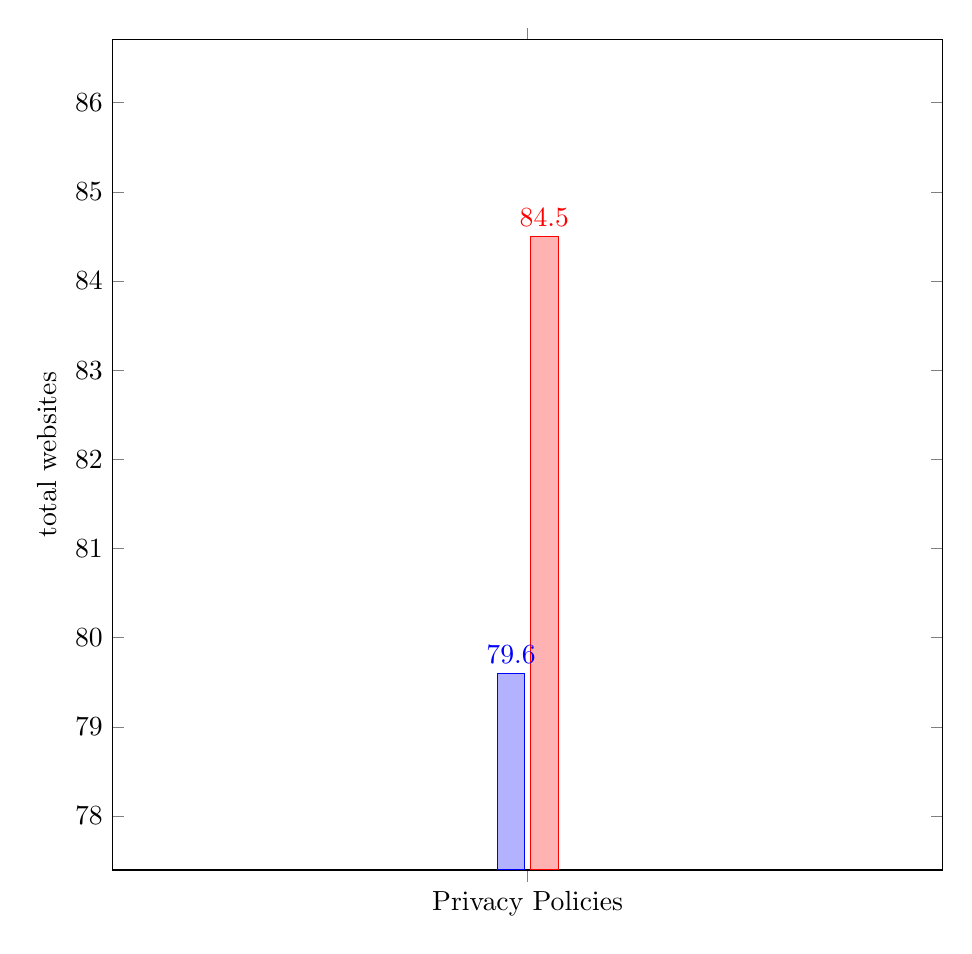
\begin{tikzpicture}
            \begin{axis}[ybar, enlargelimits=0.45, legend style = {at = {(0.5, -0.15)}, anchor=north, legend columns=-1}, ylabel={total websites}, symbolic x coords={Privacy Policies}, xtick=data, nodes near coords, nodes near coords align={vertical}, width=1\textwidth, height=1\textwidth]
                \addplot coordinates {(Privacy Policies, 79.6) };
                \addplot coordinates {(Privacy Policies, 84.5) };
        \end{axis}
        \end{tikzpicture}
        \caption{Websites offering a privacy policy page before and after the GDPR.}
        \label{fig:degeling_a}
    \end{subfigure}
    \hfill
    \begin{subfigure}[b]{0.45\textwidth}
        \centering
        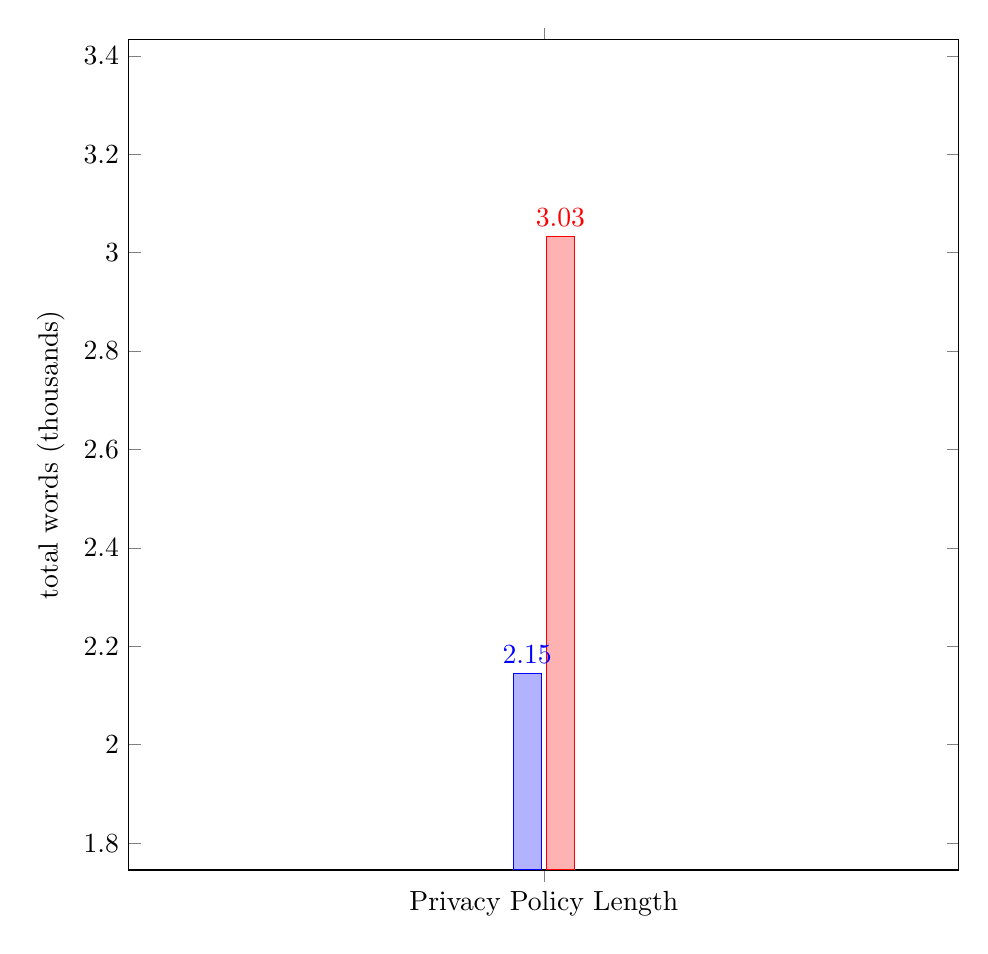
\begin{tikzpicture}
            \begin{axis}[ybar, enlargelimits=0.45, legend style={at={(1,1.3)}, anchor=north, legend columns=-1}, ylabel={total words (thousands)}, symbolic x coords={Privacy Policy Length}, xtick=data, nodes near coords, nodes near coords align={vertical}, width=1\textwidth, height=1\textwidth]
                \addplot coordinates {(Privacy Policy Length, 2.145) };
                \addplot coordinates {(Privacy Policy Length, 3.033) };
        \end{axis}
        \end{tikzpicture}
        \caption{Privacy policy length before and after the GDPR.}
        \label{fig:degeling_b}
    \end{subfigure}
    
    \begin{subfigure}[b]{0.45\textwidth}
        \centering
        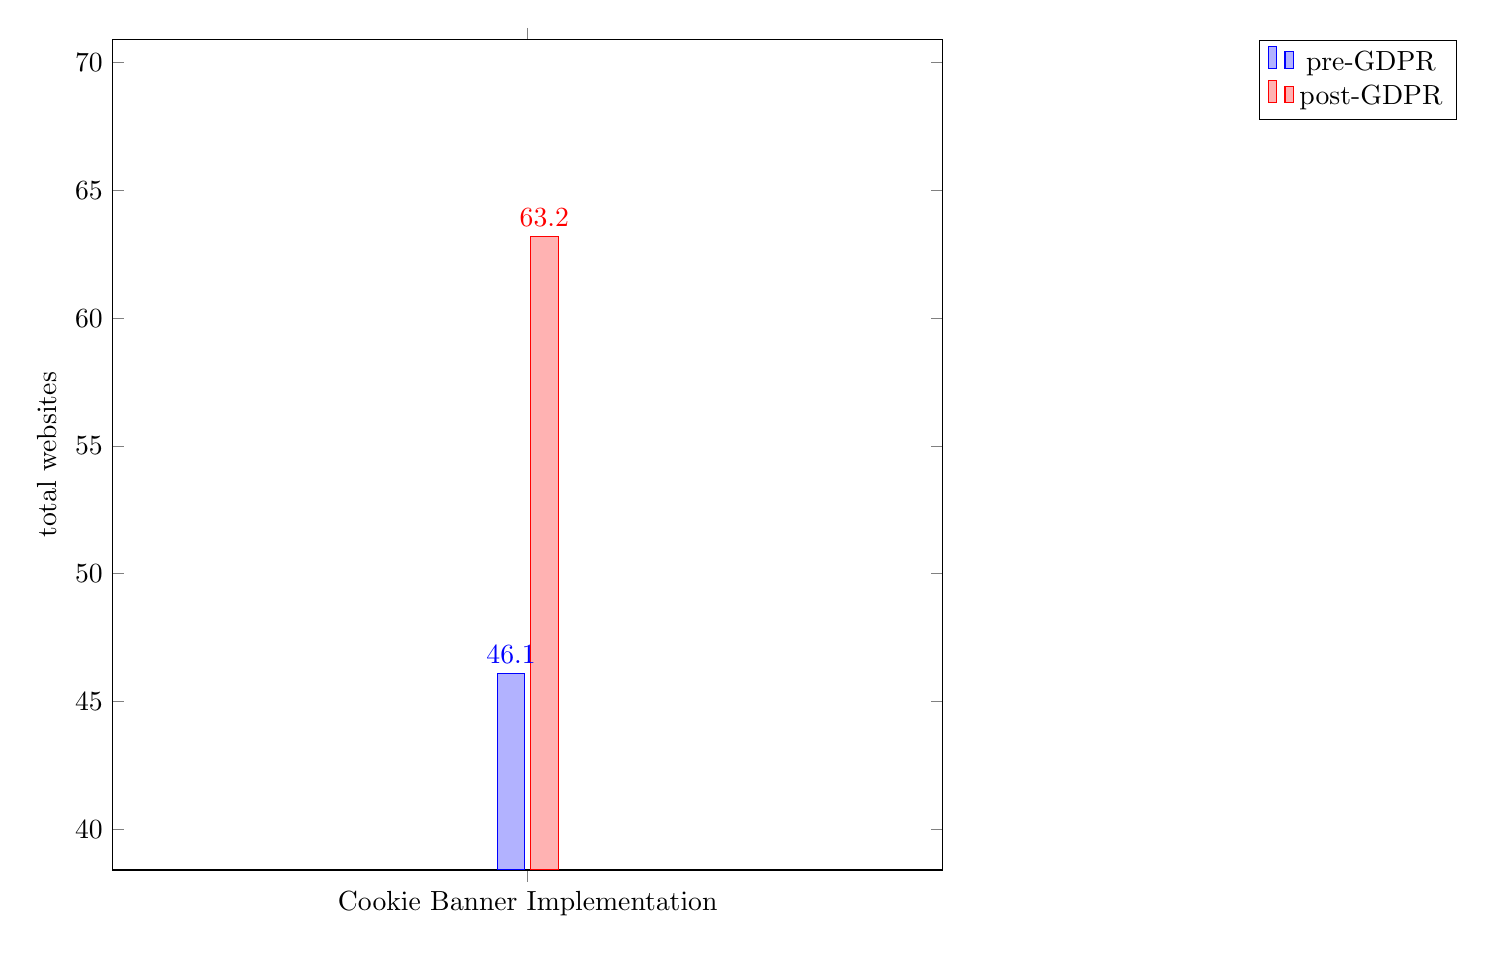
\begin{tikzpicture}
            \begin{axis}[ybar, enlargelimits=0.45, legend style={at={(1.5,1)}, anchor=north}, ylabel={total websites}, symbolic x coords={Cookie Banner Implementation}, xtick=data, nodes near coords, nodes near coords align={vertical}, width=1\textwidth, height=1\textwidth]
                \addlegendentry{pre-GDPR}
                \addplot coordinates {(Cookie Banner Implementation, 46.1) };
                \addlegendentry{post-GDPR}
                \addplot coordinates {(Cookie Banner Implementation, 63.2) };
        \end{axis}
        \end{tikzpicture}
        \caption{Cookie banner implementation before and after the GDPR.}
        \label{fig:degeling_c}
    \end{subfigure}
    \caption{The impact of GDPR on the cookie banners and privacy policies of websites, as shown by Degeling et al.}
    \label{fig:degeling}
\end{figure}

Due to all the additional regulation that came into force with the GDPR, one could assume that tracking would be impacted and therefore, websites would track their users less. However, this does not appear to be true and although users have the ability to manage their data better tracking is still ubiquitous on the internet. This was observed by Sørensen and Kosta \cite{sorensen2019before} who investigated whether the GDPR lowered the activity of third-party trackers. They did this by measuring the number of trackers before and after the GDPR went into force. The researchers used two main categories for the websites that they chose to survey. Those were the publicly-owned websites (e.g. government) and the privately-owned (e.g. entertainment) ones. The researchers surveyed websites from every country of the European Union. In total, they gathered 1,363 websites from 39 different countries which then were divided into 11 different categories. Firstly, they noticed that public websites store fewer third-party trackers than their private counterparts. However, they did not notice significant changes in the number of Third-Party Cookies, in either category, post-GDPR. Overall, Sørensen and Kosta did not observe a significant decline in the number of third-party trackers after the GDPR was put into force. Thus, the authors noted that the assumption that the GDPR is going to lead in an immediate decline in the number of TPs does not hold. 

\section{Cookie Notices and Tracking}
\label{sec:lit_review_tracking}
As Sørensen and Kosta showed, online tracking is everywhere even though legislation, such as the GDPR, is trying to contain it and give the ability to users to manage their online privacy. Furthermore, it is very hard for users to know the number of cookies that are being stored on their browsers and therefore the amount of tracking that websites are carrying out. 

Unfortunately, users are being tracked by tens, and sometimes hundreds, of Third-Party Cookies (TPs) that are being stored by the websites that they visit and these cookies are usually owned only by a handful of companies such as Google, Facebook and Twitter. The largest survey that looked at the prevalence of online tracking was conducted by Englehardt and Narayanan \cite{englehardt2016online}. They visited 1 million websites in order to detect the occurrence of online tracking on these websites. This included Third-Party Cookies (TPs), cookie synchronisation as well as fingerprinting techniques. In order to do this, the researchers developed OpenWPM, an open-source tool which allows researchers to automatically measure cookies and trackers in websites. OpenWPM allows for stateful measurements of websites. This means that websites don’t treat OpenWPM browser instances as new users. This enables measurements of trackers across multiple websites as well as detecting differences in content etc. Furthermore, because of this, OpenWPM allows researchers to load user profiles in order to provide realistic scenarios. OpenWPM automatically stores the results in an SQLite database that is made available to researchers for further analysis. Using OpenWPM, Englehardt and Narayana made over 90-million requests to their 1-million website set. Interestingly, they found that there are 81,000 web trackers on the websites that they surveyed but only 123 of those are the most prevalent. Specifically, they noted that \say{Google, Facebook, Twitter and AdNexus are the only third-party entities that are present on more than 10\% of the websites}. Moreover, the researchers found that the adoption of HTTPs technology remained low. In fact, 54\% of those trackers are HTTP only. Interestingly, they empirically confirmed the now well-known fact that news websites contain the most trackers compared to other categories within their set. The authors attributed this to the business model of these websites. Moreover, the researchers found that third-parties are \say{highly connected} by using cookie syncing. More specifically, the top 50 third-parties, which use cookie syncing technology, the probability of finding them in one of the top 100 websites is 66\%.

Online tracking using cookies, among other techniques, is rife and oftentimes extremely invasive. However, certain types of websites can employ significantly more tracking than others. For instance, political websites that lean towards the right, appear to have significantly more third-party trackers compared to their left-leaning counterparts. 

This was shown by Agarwal et al. \cite{agarwal2020stop} who researched whether hyper-partisan websites (HPWs) demonstrate any \say{particular differential behaviour} when tracking their online users. For example, they wanted to determine whether left-leaning websites track right-leaning users in a different way than the left-leaning ones do. In order to gather accurate data, the researchers curated a number of different personas that correspond to a different demographic. For gathering the data, they used the OpenWPM tool to visit the HPWs. In total, they visited 667 websites with high partisan content. After analysing the data, the researchers showed that right-leaning websites ($W^R$) set 9 more cooking on average than the left-leaning websites ($W^L$). Furthermore, they found that 72\% of the Third-Party Cookies that all HPWs store are similar to the ones that the \say{general Web} stores as well. Moreover, the researchers noted that the Alexa ranking of HPW, the $W^R$ always tends to track users more than the $W^L$. Within these results, the researchers found extreme cases where both $W^L$ and $W^R$ websites store more than 1000 cookies on a user’s device. Interestingly, the research showed that the ads shown in $W^R$ are costing 5 times more than the ads on the left-leaning websites. Overall, HPWs that tend to lean on the right, store significantly more Third-Party Cookies compared to their left-leaning counterparts with personas that realistically represent a specific demographic (e.g. Young Man), tend to receive 25\% more cookies from HPWs.

\section{Summary}
This section summarised previous research on the topic of cookie banners, privacy policies as well as internet tracking using technologies such as Third-Party Cookies and device fingerprinting. Overall, the work can be summarised in four distinct sections. These are studies on cookie banners and the privacy options that they provide to users, research on whether user location affects those cookie notices, work investigating the effects of legislation such as the GDPR and finally the prevalence of online tracking using cookies. 

However, a number of them had a particular influence on this project and especially on its research questions and methodology. Specifically, the work by Habib et al. as well as Nouwens et al. looked at the number as well as the type of privacy options provided to users by websites. This project raises similar questions but aims to do two things differently. Firstly, the objective is to survey a significantly larger dataset from 2 entirely different countries that, to our knowledge, have not been researched before. Secondly, the data gathering, as well as analysis, is conducted in an automated fashion, with manual intervention only when required, as discussed in detail in the next section of this paper. Furthermore, the tools that automate this process can be used by other researchers to conduct similar research in other countries if they wish to.

Englehardt and Narayanan focused on how widespread cookie tracking is on the internet they performed their analysis by creating OpenWPM, which is a powerful privacy measurement tool. The authors have made OpenWPM open and available to the research community. Thus, it has been extended and used by this project to crawl websites and detect cookie banners as discussed. Furthermore, the work by Eijk et al. and their CSS cookie banner scraping extension of OpenWPM has also inspired the scraping method used in this project as well. The next section will discuss in further detail the tools and methodologies used in this project in order to gather as well as analyse data. 

\end{document}